% ----------------------------------------------------------------
% AMS-LaTeX Paper ************************************************
% **** -----------------------------------------------------------
\documentclass{amsart}
\usepackage{graphicx}
% ----------------------------------------------------------------
\vfuzz2pt % Don't report over-full v-boxes if over-edge is small
\hfuzz2pt % Don't report over-full h-boxes if over-edge is small
% THEOREMS -------------------------------------------------------
\newtheorem{thm}{Theorem}[section]
\newtheorem{cor}[thm]{Corollary}
\newtheorem{lem}[thm]{Lemma}
\newtheorem{prop}[thm]{Proposition}
\theoremstyle{definition}
\newtheorem{defn}[thm]{Definition}
\theoremstyle{remark}
\newtheorem{rem}[thm]{Remark}
\numberwithin{equation}{section}
% MATH -----------------------------------------------------------
\newcommand{\norm}[1]{\left\Vert#1\right\Vert}
\newcommand{\abs}[1]{\left\vert#1\right\vert}
\newcommand{\set}[1]{\left\{#1\right\}}
\newcommand{\Real}{\mathbb R}
\newcommand{\eps}{\varepsilon}
\newcommand{\To}{\longrightarrow}
\newcommand{\BX}{\mathbf{B}(X)}
\newcommand{\A}{\mathcal{A}}
% ----------------------------------------------------------------
\begin{document}

\title{Complex Networks  - Spring 2025\\{\bf Homework 2}}%
\author{Instructor: Jia Liu}%
\date{}

%\dedicatory{}%
%\commby{}%
% ----------------------------------------------------------------

\maketitle
% ----------------------------------------------------------------
\begin{itemize}
\item DUE on 02/23/2025 11:59pm C.T.
\item You can write on the separate work sheet or type your quiz. ( Word or Latex or similar)
\item If you use the handwriting, Solutions must be neat,clear and legible.
\item If you need to scan you quiz, save it as a PDF file. Do not use jpeg, png, jpg etc. Do not submit more than one file.
\item Please check your scanned file before submission. Make sure it is readable, correct order, properly oriented. Make sure it does include all pages.
\item Please name your file as follows: $LastnameInitials-MAP5990quiz1.pdf$.If your name is Alan David Roberts, file name is $RobertsAD-MAP5990quiz1.pdf$.
\item Try to keep the file size less than 4MB.
\item You can resubmit the quiz if you want. Please specify which one is the one to be graded. Otherwise I will grade the most recent version.
\item DO NOT EMAIL me the quiz. All quizzes are submitted via Canvas.
\end{itemize}


\clearpage
\begin{enumerate}

%---------------------------------------------------------------------------------

\item Demonstrate the following for undirected networks:
\begin{enumerate}
\item A 3 regular graph must have an even number of nodes.\vspace{5cm}
\item The average degree of a tree is strictly less than 2.
\end{enumerate}

\vspace{5cm}

\item A star graph consists of a single central node with $n-1$ other nodes connected to it. 
\begin{enumerate}
\item Find the adjacency matrix of the following start network with nodes N:
\begin{figure}[h]
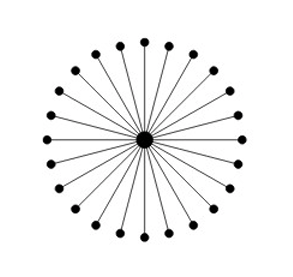
\includegraphics[width=0.4\linewidth]{stargraph.png}
\end{figure}
\item Find the largest eigenvalue of the adjacency matrix. 
\end{enumerate}

\clearpage

\item {\bf Average degree of a growing network} Assume that you are observing a growing undirected network.
The network evolves in time by this simple rules:
\begin{itemize}
\item At time $t = 1$ there is a single isolated node.
\item At each time $t > 1$ a new node is added to the network and is connected
to the existing network by a new link.
\end{itemize}
Consider the network at time $t = T$.
\begin{enumerate}
\item What is the total number of nodes N? \vspace{1cm}
\item What is the total number of links L?\vspace{1cm}
\item What is the average degree $\langle k \rangle$?\vspace{1cm}
\item  What is the average degree in the limit $T \rightarrow +\infty $?\vspace{1cm}
\end{enumerate}

\vspace{3cm}

\item One can calculate the diameter of certain types of network exactly. Assume that each of these network has network size N.
\begin{enumerate}
\item What is the diameter of a fully connected network?\vspace{1cm}
\item What is the diameter of a star network?\vspace{1cm}
\item What is the diameter of a linear chain of N nodes? \vspace{1cm}
\item What is the small world diameter property? \vspace{1cm}
\item Which of the above networks are small-world? In another word, which networks have SWDP?
\end{enumerate}
\clearpage

\item Please submit the network for your final project, including the following. This is a group work. Please discuss with your team members but each one needs to submit the individual report. 
\begin{enumerate}
\item What is your network?\vspace{1cm}
\item Where you get the data?\vspace{1cm}
\item Describe your network including the application area, size, nodes.\vspace{1cm}
\item Why you (or your team) want to study this network. 
\end{enumerate}

\end{enumerate}

\end{document}
% ----------------------------------------------------------------
